
%% bare_conf.tex
%% V1.3
%% 2007/01/11
%% by Michael Shell
%% See:
%% http://www.michaelshell.org/
%% for current contact information.
%%
%% This is a skeleton file demonstrating the use of IEEEtran.cls
%% (requires IEEEtran.cls version 1.7 or later) with an IEEE conference paper.
%%
%% Support sites:
%% http://www.michaelshell.org/tex/ieeetran/
%% http://www.ctan.org/tex-archive/macros/latex/contrib/IEEEtran/
%% and
%% http://www.ieee.org/

%%*************************************************************************
%% Legal Notice:
%% This code is offered as-is without any warranty either expressed or
%% implied; without even the implied warranty of MERCHANTABILITY or
%% FITNESS FOR A PARTICULAR PURPOSE! 
%% User assumes all risk.
%% In no event shall IEEE or any contributor to this code be liable for
%% any damages or losses, including, but not limited to, incidental,
%% consequential, or any other damages, resulting from the use or misuse
%% of any information contained here.
%%
%% All comments are the opinions of their respective authors and are not
%% necessarily endorsed by the IEEE.
%%
%% This work is distributed under the LaTeX Project Public License (LPPL)
%% ( http://www.latex-project.org/ ) version 1.3, and may be freely used,
%% distributed and modified. A copy of the LPPL, version 1.3, is included
%% in the base LaTeX documentation of all distributions of LaTeX released
%% 2003/12/01 or later.
%% Retain all contribution notices and credits.
%% ** Modified files should be clearly indicated as such, including  **
%% ** renaming them and changing author support contact information. **
%%
%% File list of work: IEEEtran.cls, IEEEtran_HOWTO.pdf, bare_adv.tex,
%%                    bare_conf.tex, bare_jrnl.tex, bare_jrnl_compsoc.tex
%%*************************************************************************

% *** Authors should verify (and, if needed, correct) their LaTeX system  ***
% *** with the testflow diagnostic prior to trusting their LaTeX platform ***
% *** with production work. IEEE's font choices can trigger bugs that do  ***
% *** not appear when using other class files.                            ***
% The testflow support page is at:
% http://www.michaelshell.org/tex/testflow/



% Note that the a4paper option is mainly intended so that authors in
% countries using A4 can easily print to A4 and see how their papers will
% look in print - the typesetting of the document will not typically be
% affected with changes in paper size (but the bottom and side margins will).
% Use the testflow package mentioned above to verify correct handling of
% both paper sizes by the user's LaTeX system.
%
% Also note that the "draftcls" or "draftclsnofoot", not "draft", option
% should be used if it is desired that the figures are to be displayed in
% draft mode.
%
\documentclass[conference]{IEEEtran}
% Add the compsoc option for Computer Society conferences.
%
% If IEEEtran.cls has not been installed into the LaTeX system files,
% manually specify the path to it like:
% \documentclass[conference]{../sty/IEEEtran}





% Some very useful LaTeX packages include:
% (uncomment the ones you want to load)


% *** MISC UTILITY PACKAGES ***
%
%\usepackage{ifpdf}
% Heiko Oberdiek's ifpdf.sty is very useful if you need conditional
% compilation based on whether the output is pdf or dvi.
% usage:
% \ifpdf
%   % pdf code
% \else
%   % dvi code
% \fi
% The latest version of ifpdf.sty can be obtained from:
% http://www.ctan.org/tex-archive/macros/latex/contrib/oberdiek/
% Also, note that IEEEtran.cls V1.7 and later provides a builtin
% \ifCLASSINFOpdf conditional that works the same way.
% When switching from latex to pdflatex and vice-versa, the compiler may
% have to be run twice to clear warning/error messages.






% *** CITATION PACKAGES ***
%
%\usepackage{cite}
% cite.sty was written by Donald Arseneau
% V1.6 and later of IEEEtran pre-defines the format of the cite.sty package
% \cite{} output to follow that of IEEE. Loading the cite package will
% result in citation numbers being automatically sorted and properly
% "compressed/ranged". e.g., [1], [9], [2], [7], [5], [6] without using
% cite.sty will become [1], [2], [5]--[7], [9] using cite.sty. cite.sty's
% \cite will automatically add leading space, if needed. Use cite.sty's
% noadjust option (cite.sty V3.8 and later) if you want to turn this off.
% cite.sty is already installed on most LaTeX systems. Be sure and use
% version 4.0 (2003-05-27) and later if using hyperref.sty. cite.sty does
% not currently provide for hyperlinked citations.
% The latest version can be obtained at:
% http://www.ctan.org/tex-archive/macros/latex/contrib/cite/
% The documentation is contained in the cite.sty file itself.






% *** GRAPHICS RELATED PACKAGES ***
%
\ifCLASSINFOpdf
  \usepackage[pdftex]{graphicx}
  % declare the path(s) where your graphic files are
  \graphicspath{{./pix/}}
  % and their extensions so you won't have to specify these with
  % every instance of \includegraphics
  \DeclareGraphicsExtensions{.pdf,.jpeg,.png,.jpg}
\else
  % or other class option (dvipsone, dvipdf, if not using dvips). graphicx
  % will default to the driver specified in the system graphics.cfg if no
  % driver is specified.
  % \usepackage[dvips]{graphicx}
  % declare the path(s) where your graphic files are
  % \graphicspath{{../eps/}}
  % and their extensions so you won't have to specify these with
  % every instance of \includegraphics
  % \DeclareGraphicsExtensions{.eps}
\fi
% graphicx was written by David Carlisle and Sebastian Rahtz. It is
% required if you want graphics, photos, etc. graphicx.sty is already
% installed on most LaTeX systems. The latest version and documentation can
% be obtained at: 
% http://www.ctan.org/tex-archive/macros/latex/required/graphics/
% Another good source of documentation is "Using Imported Graphics in
% LaTeX2e" by Keith Reckdahl which can be found as epslatex.ps or
% epslatex.pdf at: http://www.ctan.org/tex-archive/info/
%
% latex, and pdflatex in dvi mode, support graphics in encapsulated
% postscript (.eps) format. pdflatex in pdf mode supports graphics
% in .pdf, .jpeg, .png and .mps (metapost) formats. Users should ensure
% that all non-photo figures use a vector format (.eps, .pdf, .mps) and
% not a bitmapped formats (.jpeg, .png). IEEE frowns on bitmapped formats
% which can result in "jaggedy"/blurry rendering of lines and letters as
% well as large increases in file sizes.
%
% You can find documentation about the pdfTeX application at:
% http://www.tug.org/applications/pdftex





% *** MATH PACKAGES ***
%
%\usepackage[cmex10]{amsmath}
% A popular package from the American Mathematical Society that provides
% many useful and powerful commands for dealing with mathematics. If using
% it, be sure to load this package with the cmex10 option to ensure that
% only type 1 fonts will utilized at all point sizes. Without this option,
% it is possible that some math symbols, particularly those within
% footnotes, will be rendered in bitmap form which will result in a
% document that can not be IEEE Xplore compliant!
%
% Also, note that the amsmath package sets \interdisplaylinepenalty to 10000
% thus preventing page breaks from occurring within multiline equations. Use:
%\interdisplaylinepenalty=2500
% after loading amsmath to restore such page breaks as IEEEtran.cls normally
% does. amsmath.sty is already installed on most LaTeX systems. The latest
% version and documentation can be obtained at:
% http://www.ctan.org/tex-archive/macros/latex/required/amslatex/math/





% *** SPECIALIZED LIST PACKAGES ***
%
%\usepackage{algorithmic}
% algorithmic.sty was written by Peter Williams and Rogerio Brito.
% This package provides an algorithmic environment fo describing algorithms.
% You can use the algorithmic environment in-text or within a figure
% environment to provide for a floating algorithm. Do NOT use the algorithm
% floating environment provided by algorithm.sty (by the same authors) or
% algorithm2e.sty (by Christophe Fiorio) as IEEE does not use dedicated
% algorithm float types and packages that provide these will not provide
% correct IEEE style captions. The latest version and documentation of
% algorithmic.sty can be obtained at:
% http://www.ctan.org/tex-archive/macros/latex/contrib/algorithms/
% There is also a support site at:
% http://algorithms.berlios.de/index.html
% Also of interest may be the (relatively newer and more customizable)
% algorithmicx.sty package by Szasz Janos:
% http://www.ctan.org/tex-archive/macros/latex/contrib/algorithmicx/




% *** ALIGNMENT PACKAGES ***
%
\usepackage{array}
% Frank Mittelbach's and David Carlisle's array.sty patches and improves
% the standard LaTeX2e array and tabular environments to provide better
% appearance and additional user controls. As the default LaTeX2e table
% generation code is lacking to the point of almost being broken with
% respect to the quality of the end results, all users are strongly
% advised to use an enhanced (at the very least that provided by array.sty)
% set of table tools. array.sty is already installed on most systems. The
% latest version and documentation can be obtained at:
% http://www.ctan.org/tex-archive/macros/latex/required/tools/


%\usepackage{mdwmath}
%\usepackage{mdwtab}
% Also highly recommended is Mark Wooding's extremely powerful MDW tools,
% especially mdwmath.sty and mdwtab.sty which are used to format equations
% and tables, respectively. The MDWtools set is already installed on most
% LaTeX systems. The lastest version and documentation is available at:
% http://www.ctan.org/tex-archive/macros/latex/contrib/mdwtools/


% IEEEtran contains the IEEEeqnarray family of commands that can be used to
% generate multiline equations as well as matrices, tables, etc., of high
% quality.


%\usepackage{eqparbox}
% Also of notable interest is Scott Pakin's eqparbox package for creating
% (automatically sized) equal width boxes - aka "natural width parboxes".
% Available at:
% http://www.ctan.org/tex-archive/macros/latex/contrib/eqparbox/





% *** SUBFIGURE PACKAGES ***
%\usepackage[tight,footnotesize]{subfigure}
% subfigure.sty was written by Steven Douglas Cochran. This package makes it
% easy to put subfigures in your figures. e.g., "Figure 1a and 1b". For IEEE
% work, it is a good idea to load it with the tight package option to reduce
% the amount of white space around the subfigures. subfigure.sty is already
% installed on most LaTeX systems. The latest version and documentation can
% be obtained at:
% http://www.ctan.org/tex-archive/obsolete/macros/latex/contrib/subfigure/
% subfigure.sty has been superceeded by subfig.sty.



%\usepackage[caption=false]{caption}
%\usepackage[font=footnotesize]{subfig}
% subfig.sty, also written by Steven Douglas Cochran, is the modern
% replacement for subfigure.sty. However, subfig.sty requires and
% automatically loads Axel Sommerfeldt's caption.sty which will override
% IEEEtran.cls handling of captions and this will result in nonIEEE style
% figure/table captions. To prevent this problem, be sure and preload
% caption.sty with its "caption=false" package option. This is will preserve
% IEEEtran.cls handing of captions. Version 1.3 (2005/06/28) and later 
% (recommended due to many improvements over 1.2) of subfig.sty supports
% the caption=false option directly:
\usepackage[caption=false,font=footnotesize]{subfig}
%
% The latest version and documentation can be obtained at:
% http://www.ctan.org/tex-archive/macros/latex/contrib/subfig/
% The latest version and documentation of caption.sty can be obtained at:
% http://www.ctan.org/tex-archive/macros/latex/contrib/caption/




% *** FLOAT PACKAGES ***
%
\usepackage{fixltx2e}
% fixltx2e, the successor to the earlier fix2col.sty, was written by
% Frank Mittelbach and David Carlisle. This package corrects a few problems
% in the LaTeX2e kernel, the most notable of which is that in current
% LaTeX2e releases, the ordering of single and double column floats is not
% guaranteed to be preserved. Thus, an unpatched LaTeX2e can allow a
% single column figure to be placed prior to an earlier double column
% figure. The latest version and documentation can be found at:
% http://www.ctan.org/tex-archive/macros/latex/base/



%\usepackage{stfloats}
% stfloats.sty was written by Sigitas Tolusis. This package gives LaTeX2e
% the ability to do double column floats at the bottom of the page as well
% as the top. (e.g., "\begin{figure*}[!b]" is not normally possible in
% LaTeX2e). It also provides a command:
%\fnbelowfloat
% to enable the placement of footnotes below bottom floats (the standard
% LaTeX2e kernel puts them above bottom floats). This is an invasive package
% which rewrites many portions of the LaTeX2e float routines. It may not work
% with other packages that modify the LaTeX2e float routines. The latest
% version and documentation can be obtained at:
% http://www.ctan.org/tex-archive/macros/latex/contrib/sttools/
% Documentation is contained in the stfloats.sty comments as well as in the
% presfull.pdf file. Do not use the stfloats baselinefloat ability as IEEE
% does not allow \baselineskip to stretch. Authors submitting work to the
% IEEE should note that IEEE rarely uses double column equations and
% that authors should try to avoid such use. Do not be tempted to use the
% cuted.sty or midfloat.sty packages (also by Sigitas Tolusis) as IEEE does
% not format its papers in such ways.





% *** PDF, URL AND HYPERLINK PACKAGES ***
%
%\usepackage{url}
% url.sty was written by Donald Arseneau. It provides better support for
% handling and breaking URLs. url.sty is already installed on most LaTeX
% systems. The latest version can be obtained at:
% http://www.ctan.org/tex-archive/macros/latex/contrib/misc/
% Read the url.sty source comments for usage information. Basically,
% \url{my_url_here}.





% *** Do not adjust lengths that control margins, column widths, etc. ***
% *** Do not use packages that alter fonts (such as pslatex).         ***
% There should be no need to do such things with IEEEtran.cls V1.6 and later.
% (Unless specifically asked to do so by the journal or conference you plan
% to submit to, of course. )


% correct bad hyphenation here
\hyphenation{op-tical net-works semi-conduc-tor}


\begin{document}
\title{FlatFish -- A compact AUV for sub sea resident inspection tasks}

\author{\IEEEauthorblockN{Jan Albiez\IEEEauthorrefmark{1}\IEEEauthorrefmark{2}, Sylvain Joyeux\IEEEauthorrefmark{1}, Christopher Gaudig\IEEEauthorrefmark{2}, Jens Hilljegerdes\IEEEauthorrefmark{3}, Sven Kroffke\IEEEauthorrefmark{3}, \\
		Christian Schoo\IEEEauthorrefmark{2}, Sascha Arnold\IEEEauthorrefmark{2}, Geovane Mimoso\IEEEauthorrefmark{1}, Rafael Saback\IEEEauthorrefmark{1}, Joao Neto\IEEEauthorrefmark{1}, Diego Cesar\IEEEauthorrefmark{1}, \\
                Gustavo Neves\IEEEauthorrefmark{1}, Thomio Watanabe\IEEEauthorrefmark{1},
	   and Frank Kirchner\IEEEauthorrefmark{2}\IEEEauthorrefmark{2}\IEEEauthorrefmark{1}}
	\IEEEauthorblockA{\IEEEauthorrefmark{1}BIR --  Brasilian Institute for Robotics, SENAI CIMATEC, Salvador, Bahia, Brasil, Email: jan.albiez@fieb.org.br}
	\IEEEauthorblockA{\IEEEauthorrefmark{2}RIC -- Robotics Innovation Center, DFKI Deutsches Forschungszentrum f\"ur k\"unstliche Intelligenz, Bremen, Germany}
	\IEEEauthorblockA{\IEEEauthorrefmark{3}Arbeitsgruppe Robotik, Universit\"at Bremen, Bremen, Germany}
	}

% author names and affiliations
% use a multiple column layout for up to three different
% affiliations
%\author{\IEEEauthorblockN{Michael Shell}
%\IEEEauthorblockA{School of Electrical and\\Computer Engineering\\
%Georgia Institute of Technology\\
%Atlanta, Georgia 30332--0250\\
%Email: http://www.michaelshell.org/contact.html}
%\and
%\IEEEauthorblockN{Homer Simpson}
%\IEEEauthorblockA{Twentieth Century Fox\\
%Springfield, USA\\
%Email: homer@thesimpsons.com}
%\and
%\IEEEauthorblockN{James Kirk\\ and Montgomery Scott}
%\IEEEauthorblockA{Starfleet Academy\\
%San Francisco, California 96678-2391\\
%Telephone: (800) 555--1212\\
%Fax: (888) 555--1212}}

% conference papers do not typically use \thanks and this command
% is locked out in conference mode. If really needed, such as for
% the acknowledgment of grants, issue a \IEEEoverridecommandlockouts
% after \documentclass

% for over three affiliations, or if they all won't fit within the width
% of the page, use this alternative format:
% 
%\author{\IEEEauthorblockN{Michael Shell\IEEEauthorrefmark{1},
%Homer Simpson\IEEEauthorrefmark{2},
%James Kirk\IEEEauthorrefmark{3}, 
%Montgomery Scott\IEEEauthorrefmark{3} and
%Eldon Tyrell\IEEEauthorrefmark{4}}
%\IEEEauthorblockA{\IEEEauthorrefmark{1}School of Electrical and Computer Engineering\\
%Georgia Institute of Technology,
%Atlanta, Georgia 30332--0250\\ Email: see http://www.michaelshell.org/contact.html}
%\IEEEauthorblockA{\IEEEauthorrefmark{2}Twentieth Century Fox, Springfield, USA\\
%Email: homer@thesimpsons.com}
%\IEEEauthorblockA{\IEEEauthorrefmark{3}Starfleet Academy, San Francisco, California 96678-2391\\
%Telephone: (800) 555--1212, Fax: (888) 555--1212}
%\IEEEauthorblockA{\IEEEauthorrefmark{4}Tyrell Inc., 123 Replicant Street, Los Angeles, California 90210--4321}}




% use for special paper notices
%\IEEEspecialpapernotice{(Invited Paper)}




% make the title area
\maketitle


\begin{abstract}
%\boldmath
The abstract goes here.
\end{abstract}
% IEEEtran.cls defaults to using nonbold math in the Abstract.
% This preserves the distinction between vectors and scalars. However,
% if the conference you are submitting to favors bold math in the abstract,
% then you can use LaTeX's standard command \boldmath at the very start
% of the abstract to achieve this. Many IEEE journals/conferences frown on
% math in the abstract anyway.

% no keywords




% For peer review papers, you can put extra information on the cover
% page as needed:
% \ifCLASSOPTIONpeerreview
% \begin{center} \bfseries EDICS Category: 3-BBND \end{center}
% \fi
%
% For peerreview papers, this IEEEtran command inserts a page break and
% creates the second title. It will be ignored for other modes.
\IEEEpeerreviewmaketitle



\section{Introduction}

Underwater structures like oil and gas production systems or the foundation of buildings,
piers and off-shore wind facilities, have to be regularly inspected to evaluate the state
of the structure and to plan future interventions for repair and maintenance. These
inspections are currently done by remotely operated vehicles (ROVs) or, if water depth and
availability allows it, by divers. Due to the fact that Inspections of this kind need a
special support vessel, they are time-consuming, expensive, need to be planned a long time
in advance and rely on good weather conditions and seasonal constraints (e.g.~not during
hurricane season or winter storms).

Especially when looking at the sub-sea operations of the oil and gas industry, being able
to inspect the sub-sea part of an asset regularly and/or on demand plays a key role for
sub-sea asset integrity assurance (SIA) and integrity management. The key informations
needed from of the inspections are the general structural integrity and close visual data
(also known as close visual inspection CVI). The former can be acquired by using sonars
from a greater distance for the latter a camera has to be brought close to the structure.
The capability to get information of the current state of any sub-sea equipment within the
field whenever the need for an assessment arises, allows for much safer operations and a
reduction of the operational expenditures (OPEX) due to the ability to better plan asset
maintenance. While this holds already true for current offshore assets, it becomes crucial
for the planned deep sea assets or in future fields with more complex sea floor production
systems.

These kind of inspection are logistically and financially not possible to execute with
ROVs since that would require the continuous presence of a ROV support vessel in the
field. There are a few rare installation with ROVs deployed by FPSOs, but the limitation
of the tether length limits these operational radius in an area around the FPSO. The
solution is the usage of autonomous underwater vehicles (AUVs) for in-field inspection.
Already \cite{gamechanger07} predicted the increase of AUV capabilities and their usage in
tasks beyond the classic bathymetry.

AUV systems capable of delivering the desired inspection data need enhanced capabilities.
The robot must be able to bring its cameras and lights close to the inspection target
without damaging the structure. This requires a ROV like maneuverability combined with an
control systems maintaining safe operations. This hovering ability is one of the key
capabilities which is commonly used to distinguish the bathymetry class AUVs from the
inspection class AUVs.

To guarantee that at any given time a inspection of the assets sub-sea structures can be
done, the AUV has to be readily available 24/7. Since deck space on platforms and FPSO is
generally tight and to reduce the influence of the weather on operations, the solution is
to operate the AUV \textit{sub-sea resident}. Sub sea resident within the AUV context
means, that the robot has a dedicated docking station on the sea floor within the asset.
This docking station is connected to the top side facilities of the asset. While in the
docking station the AUV can be charged and data can be downloaded from the AUV and mission
information can be uploaded to the AUV. When an inspection is required the mission is
created on shore or top side and transmitted to the AUV. The AUV then leaves the docking
station, executes the mission and returns to the docking station to recharge the batteries
and transfer the inspection data.

Sub sea residence is not a new concept. The idea is being passed around in research and
development already for some time (e.g.~\cite{mcleod2011}). But until now the technology
for actually implementing a sub-sea resident vehicle has not been available. Sub sea
residency originally came out of the oceanographic research, where its intend was to
expand the ranges of long-term environmental monitoring. World wide there are a couple of
projects going on which have the usage of resident AUVs in the mid- to long-term plan,
e.g.~\cite{german2012} or \cite{soltwedel2013}.

The requirements for a sub-sea resident AUV and its supporting infrastructure are high.
All components have to be robust enough to be able to function even when being exposed to
the deep sea environment for a longer time. This includes for example corrosion,
bio-fouling, degradation of seals and the blockage of moving parts like thruster and
locking mechanisms by sand or other dirt. The AUV as well as the infrastructure has to be
designed in a way which on one hand addresses aforementioned problems and on the other
hand allows for quick and cost efficient maintenance.

\subsection{Project FlatFish}

The FlatFish project is an initiative between BG Group Brazil and the Brazilian Institute
for Robotics (BIR) in Salvador and is funded through the Brazilian Government R\&D levy,
which requires that 1\% of gross production revenue from large Brazilian oil and gas
fields to be invested in R\&D in Brazil.

FaltFish aims at the development of a sub-sea resident inspection AUV. The project is part
of a long-term research road-map of BG Group Brazil in the area of robotic for oil and gas
production. The development of the AUV is devided in two phases: In the first phase the
development infrastructure in Brazil will be developed, the AUV will be designed and
integrated, and the first inspection tests will be conducted inshore of the coast of
Salvador, Brazil and in the maritime test tank at DFKI in Bremen, Germany, The second
phase will concentrate on extended offshore trials of the complete system, including the
docking station, within an asset of BG Group. Currently the project is at the end of the
first phase.

During a workshop between BG Group, BIR and DFKI at the begin of the FlatFish project the
scenario and the principal design parameters were defined. The scenario was defines as the
following:

\begin{enumerate}
    \item The AUV resides with in a docking station on the sea floor
    \item Top side sends a mission to inspect a specific structure within the asset,
        e.g.~a mainfold or a SSIV
    \item FlatFish leaves the docking station, and flies to the specified structure using
        pipelines and other sub-sea structures as external references
    \item While in transit FlatFish uses its on-board sensors to record data of the assets
        status (e.g.~pipelines or debris) and to avoid obstacles
    \item At the inspection target FlatFish uses an advanced camera system to do a close
        visual inspection of the complete structure
    \item FlatFish returns to the docking station using the same navigation system as
        going to the structure
    \item In the docking station the batteries are recharged, the data downloaded to
        top-side and a high resolution video linked 3D model is created as inspection
        result.
\end{enumerate}

With this in mind the basic requirements for the FlatFish AUV were set to the following:

\begin{itemize}
    \item Compact design with hovering capabilities
    \item Materials and mechanical design that allow for a long term sub-sea deployment
    \item Extended sensor suite including for highly detailed visual inspection.
    \item Multi-modal navigation system tailored to use the assets structure as landmarks
    \item Multiple tracking systems e.g. pipeline tracking, cable tracking, structure
        tracking
    \item On-line 3D reconstruction for adaptive inspection coverage and off-line dense 3D
        reconstruction with referencing between video data and 3D model
\end{itemize}

This paper focuses on the FlatFish AUV. The developments within the project are set into
the current state of the art on inspection class AUVs and the design of the AUV is
presented.

%%%%%%% here because of layout reasons
\begin{table}[!t]
% increase table row spacing, adjust to taste
\renewcommand{\arraystretch}{1.3}
% if using array.sty, it might be a good idea to tweak the value of
% \extrarowheight as needed to properly center the text within the cells
\caption{FlatFish -- Technical Data}
\label{tab:tech}
\centering
% Some packages, such as MDW tools, offer better commands for making tables
% than the plain LaTeX2e tabular which is used here.
\begin{tabular}{|l|l|}
\hline
Depth rating 	  & 300 m \\ \hline

Weight (in air)		& 275 kg \\ \hline

Size (LWH)			&	220 cm x 105 cm x 50 cm \\ \hline

Propulsion			& 6x 60N Enitech ring thrusters \\
 & (120N in each direction) \\ \hline

Battery	 			&  Lithium-Ion battery 5,8 kWh (11,6 kWh) @ 48V\\ \hline 

Communication & Rock7mobile RockBlock Iridium satellite modem (1,6 GHz) \\
(surface) 		& Digi XBee-Pro-868 (868 MHz)\\
 & ubiquiti PicoStation M2 HP WLAN-Modul (2,4 GHz) \\ \hline

Communication & Evologics S2CR 48/78 kHz \\
(submerged)	&	usable as USBL transponder \\ \hline

Communication & 10 GBit/s optical fibre \\
(tethered)			& 1 GBit/s Cat5e (max. 50m) \\ \hline


Light	& 4x Bowtech LED-K-3200 (3200 lumen each) \\ \hline

Laser Line & 2x Picotronic LD532-20-3(20x80)45-PL line laser \\
projector & 20mW each @ 532nm \\ \hline

Sonar	& BlueView MB1350-45 Multibeam Profiler (inspection sonar) \\
 & Tritech Gemini 720i Multibeam Imager (navigation sonar) \\
 & 2x Tritech Micron Sonar (obstacle avoidance) \\ \hline
  
Camera	& 4x Basler ace acA2040-gc25 \\
	& 2048x2048 at 25 frames/s, colour, GigabitEthernet \\\hline
	
Depthsensor & Paroscientific 8CDP700-I \\ \hline

INS/AHRS & KVH 1750 IMU \\ \hline

DVL &	Rowe SeaProfiler DualFrequency 300/1200 kHz \\ \hline
\end{tabular}
\end{table}

\begin{figure*}[!t]
	\begin{center}
		\centering
		\subfloat[bottom view]{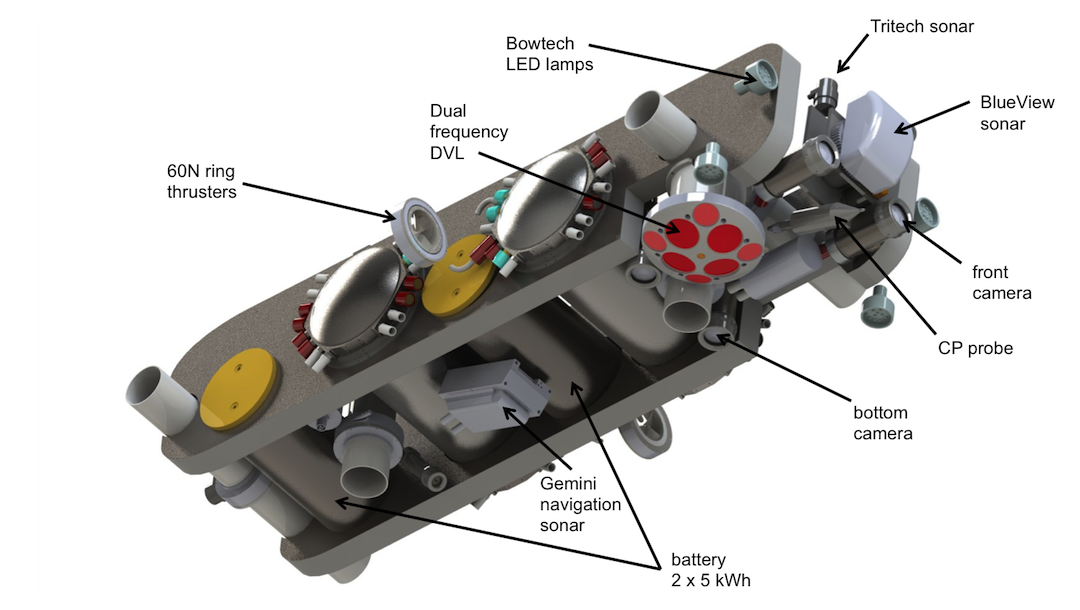
\includegraphics[width=0.5\textwidth]{flatfish_unten}}
		\hfil
		\subfloat[top view]{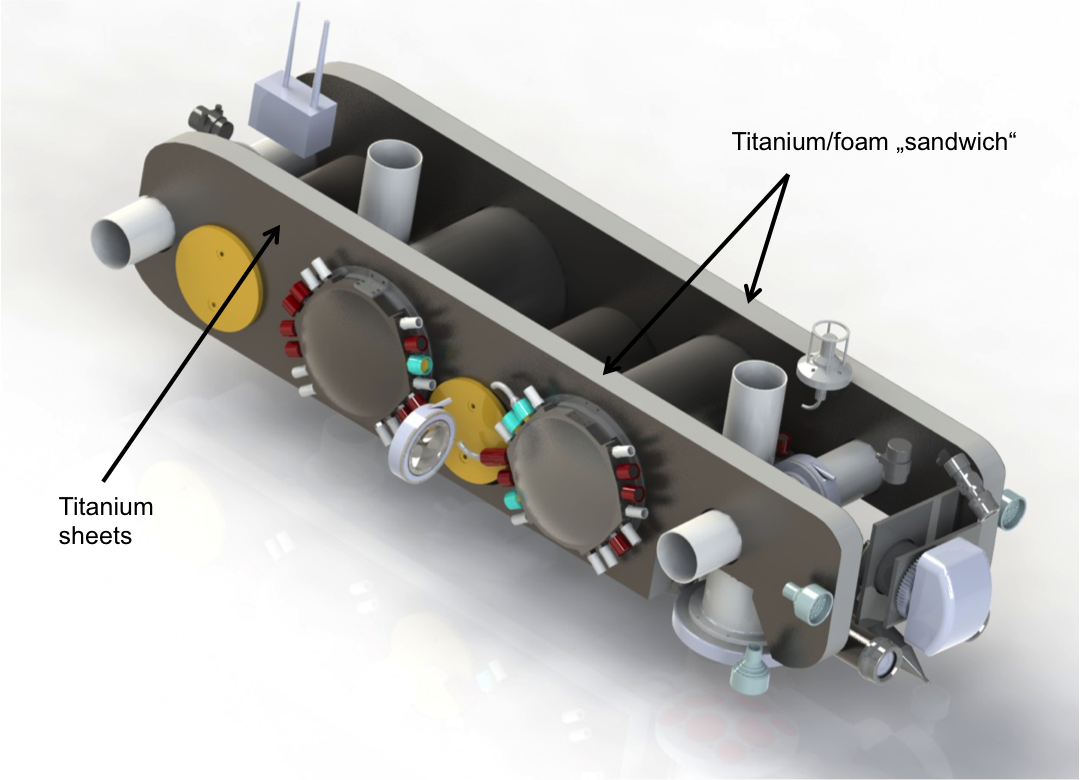
\includegraphics[width=0.5\textwidth]{flatfish_oben}}
		\caption{Overview of the principal placement of the FlatFishs components (sensors, thrusters etc.)}
		\label{fig:sensor_placement}
	\end{center}
\end{figure*}
%%%%%%%

\section{Inspection Class AUVs}

The primary tasks for autonomous underwater vehicles has always been data collection.
Initially AUVs were designed to enhance the quality of sonar based wide area surveys by
operating closer to the ground and without the influence of waves. Up to this day
facilitating high-resolution bathymetric maps is still the primary application for AUVs.
Other wide area operations are the search for objects such as flight recorders (see
\cite{purcell2011}) or mine hunting (see \cite{Couillard2012}). AUVs designed to do these
kind of tasks commonly only use one propeller and control planes and therefore lack the
ability to \textit{hover}, meaning that they can't stay in one place like ROVs. The
ability to hover is a key requirement to do inspection tasks on complex structures.
Therefore this ability distinguishes inspection class AUVs from mapping systems.

In recent years several AUV manufactures designed prototypical modifications of their
mapping AUVs to do inspection tasks, e.g.~the modified REMUS 500 presented in
\cite{packard2010}. All of this modifications have in common, that hovering is relatively
expensive energy wise, so inspections which mainly rely on ROV like motions are not
feasible with these systems.

SubSea 7s autonomous inspection vehicle (AIV) \cite{AIV} comes close to the requirements
defined for the FlatFish project. Nevertheless the AIV mainly operates sonar based and
keeps longer distance to the inspection target and lacks additionally lacks the required
high resolution video system.

Lockheed Martins Marlin \cite{Marlinmk1} is a huge AUV primarily designed for carrying a
bulky 3D imaging sonar. It has been used to do optical surveys as well (see
\cite{mcleod2013}) but with mixed results. There has been some tries to use the Saab
Seaeye Sabertooth \cite{johansson2010} as inspection class AUV, but up it suffers from the
same size problems as the Marlin. 

There are several prototypes and single systems used in robotic or marine research.
Examples are the Italian TriMares \cite{cruz2011} used to evaluate dam inspection by AUVs,
the Spanish Girona 500 vehicle \cite{ribas2012} used in different European projects and
the Sentry AUV of the Woods Hole Oceanographic Institution in the USA, best known for its
work during the Deepwater Horizon accident \cite{Kinsey2011}. All these system have in
common, that they are unique solutions with special research interests.

A special case currently being under development are so called \textit{hybrid} ROVs, which
basically are hovering AUVs which are remotely controlled via a thin optical fiber during
the inspection/scientific part of their mission. The first known vehicle of this kind was
the deep diving NEREUS \cite{bowen2009}. An example for a resent system is the HROV
\cite{meinecke2011} of the German MARUM.

The work in FlatFish is based on the long experience of the DFKI RIC on the design of
inspection AUVs. It mainly builds upon the operational experience made with DAGON
\cite{hildebrandt2012} and on the mechatronic system of LENG \cite{hildebrandt2013}.

\section{Brasilian-German Development}

FlatFish is developed in a joint effort between the Robotics Innovation Center (RIC) of
DFKI in Bremen, Germany and the Brazilian Institute for Robotics (BIR) in Salvador,
Brazil. This co-operation opens the unique opportunity to combine the indoor testing
facilities and the experience on autonomous underwater robots in Bremen with the extended
testing opportunities and the emerging commercial and scientific market in Brazil.

The key elements of this co-operation within the project are the testing facilities which
complement each other, the joint development of hard and software and the training of
researchers and personnel.

The center of the maritime exploration
hall\footnote{http://robotik.dfki-bremen.de/en/research/research-facilities/maritime-exploration-hall.html}
at the facilities of DFKI RIC in Bremen is a 3.5 million liter salt water test tank. This
tank allows for comprehensive tests of systems and control algorithms in a completely
controlled and safe environment. It is big enough for FlatFish to operate freely.

The coastal waters around Salvador have an average depth of approximately 30m and offer
variety of different testing environments, close to offshore conditions with respect to
visibility and currents. The weather  allows for a nearly year around testing with only a
short time in autumn (May to mid July) where high waves and thunderstorms can limit the
ability to test. 

Both locations will have their own FlatFish AUV. The first is being built in Bremen, the
second will be integrated in Salvador. Having two vehicle allows a seamless test,
evaluation and improvement of algorithms, hardware and operational procedures. For example
can a new algorithm for sensor processing be tested in the clear water environment at
Bremen and its principal functionality can be verified before it is tested in the ocean
environment in Salvador. The results of the tests in Salvador can then be analyzed at both
locations, any problems can be identified and the testing cycle can start again. With both
location typed working in parallel this cycle can be very quick and efficient.

Working in a trans-continental co-operation forced the team to establish modern methods of
distributed development, change management, issue tracking, document management and
communication. The primary tool for co-ordinating the development work is
github\footnote{https://github.com/} which already brings all the tools needed to manage a
distribute team of software developers. Additional to github a built server is used to
verify the current state of the software integration and
runrun.it\footnote{https://runrun.it/} is used to manage the tasks of the team members and
co-ordinate the work between them. 

\section{The FlatFish AUV}

\subsection{Mechatronic Design}


\begin{figure}[!t]
	\centering
	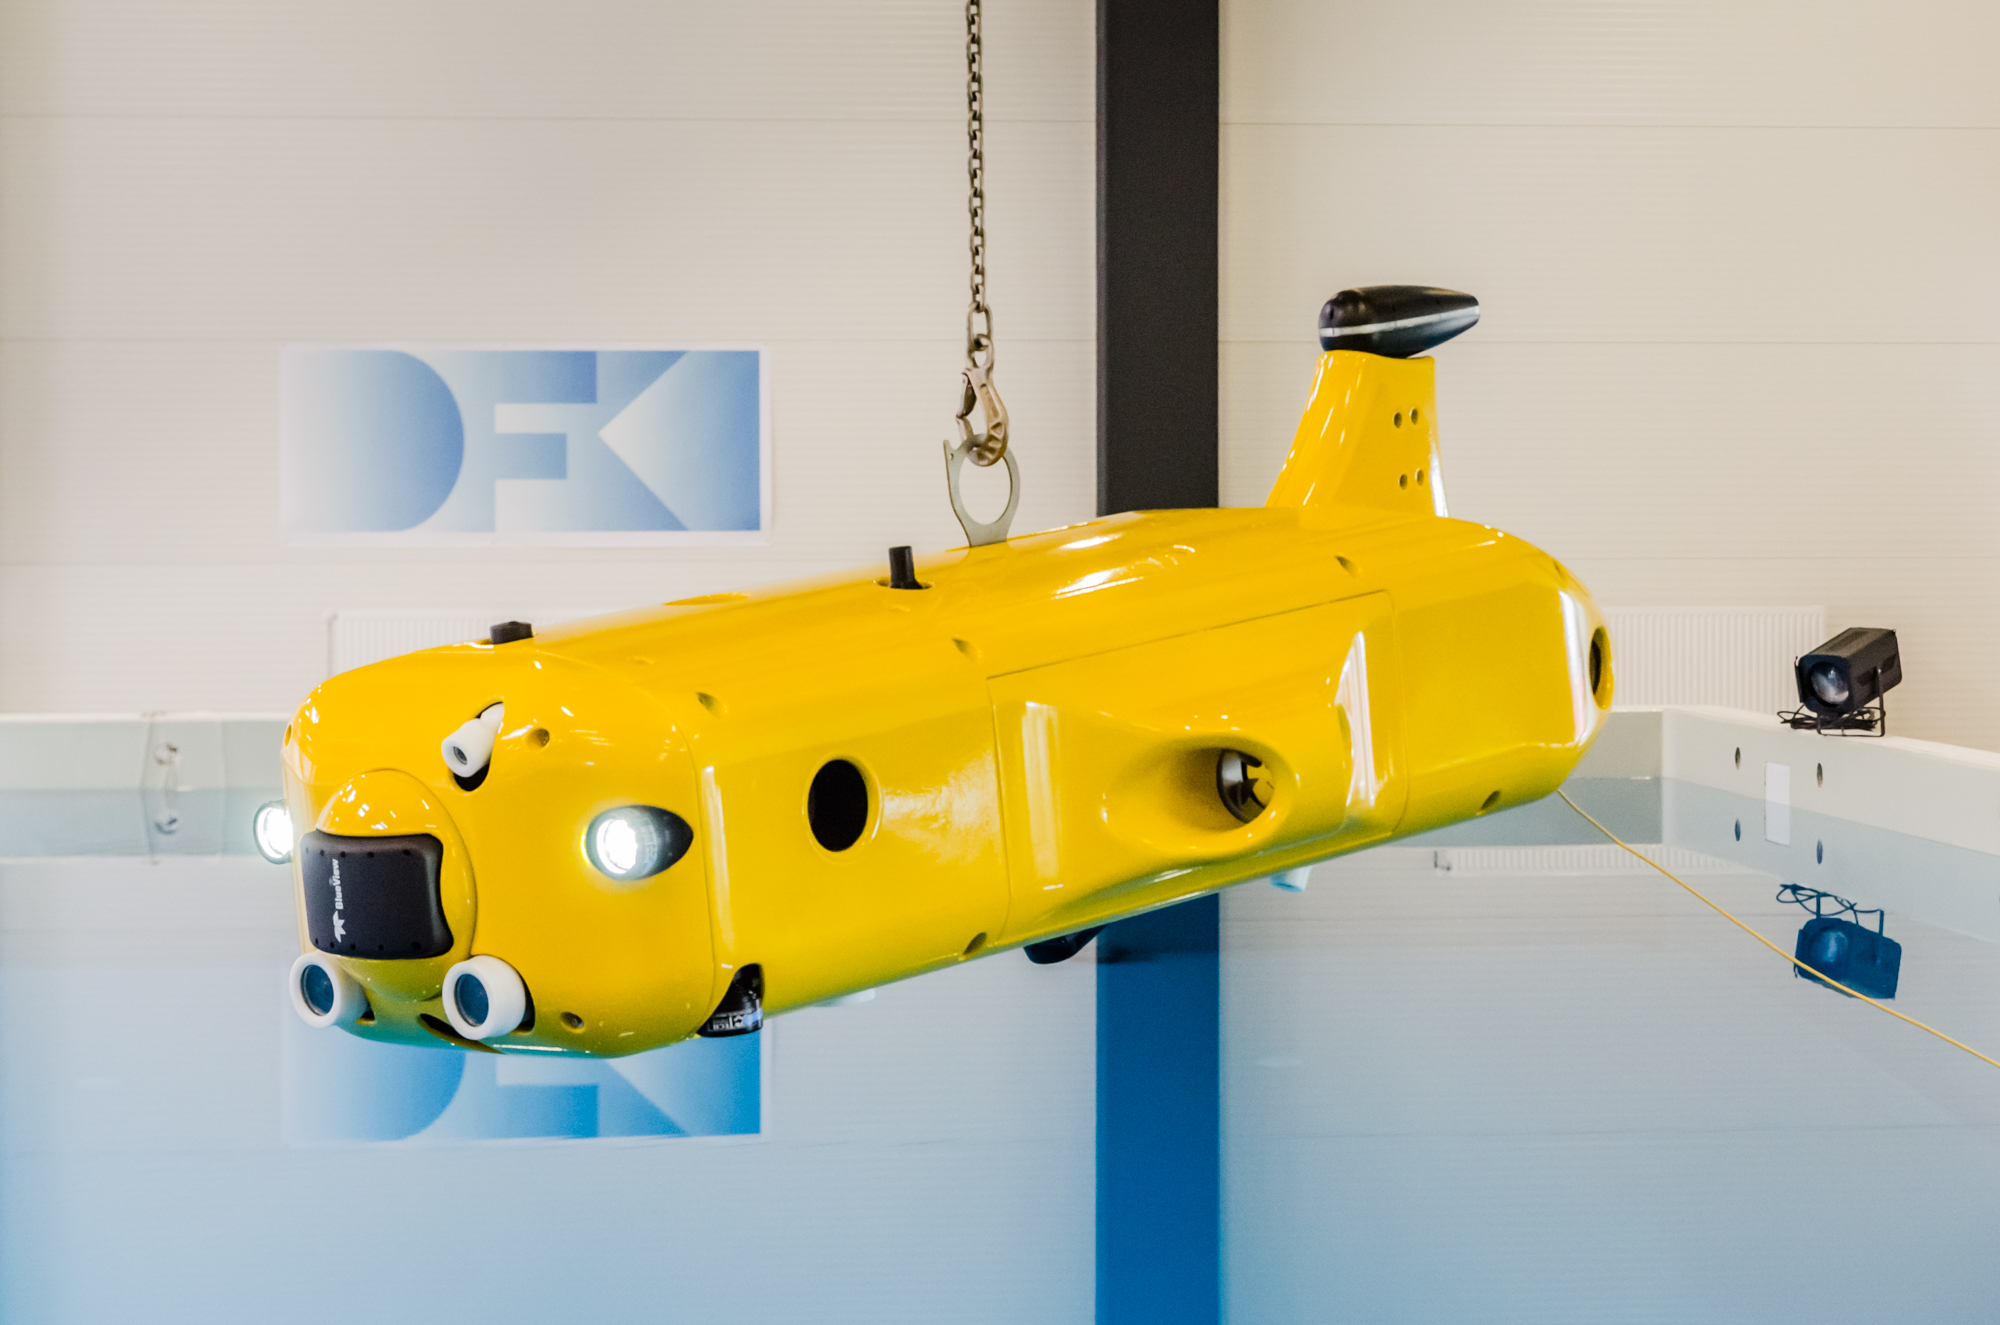
\includegraphics[width=0.9\columnwidth]{FlatFish-1.jpg}
	\caption{The completely integrated FlatFish at the DFKI RIC test facilities in Bremen, Germany.}
	\label{fig:flatfish1}
\end{figure}


\subsection{Software Architecture}

The vehicle's software architecture is based on the Robot Construction Kit
(Rock\footnote{http://rock-robotics.org/}), a component-based software integration
framework for robotics. The work done to use Rock on FlatFish is a continuation of
previous work, to which some of the authors participated, on other AUVs~\cite{albiez2010}
and H-ROVs~\cite{meinecke2013}.

From the point of view of the vehicle development, Rock provides the common type of tools
and services that is nowadays considered standard: visualization, logging (saving data)
and log replay (passing logged data to live components for testing) and state monitoring.
Where Rock differentiates itself is in its focus on robustness.

Rock's architecture design supports the integration and \emph{coordination} of software
components that have a single purpose~\cite{Joyeux2013}, that is have a well-defined function that is as
stateless as possible. This is in contrast with the common approach of ``fat components'',
whose behaviour very commonly depends on a lot of internal state, and is therefore hard to
assess externally. The components in the FlatFish architecture are meant to be designed
for a single purpose, which makes external diagnostic easier, and allow to make them
\emph{fail early}. The handling of these faults is then delegated to the system's
coordination layer, Syskit\cite{Joyeux2011}.

Syskit is a model-based approach designed to handle a component-based approach to data
processing in the robotic context~\ref{fig:sw_arch}. In addition to its diagnostic and fault recovery
aspects, it allows to design the different configurations of the system's component
networks, building a \emph{Behaviour Pool}, and then combine them in more complex systems
(correct-by-construction). At runtime, these various subsystems can then be switched on or
off when needed by the \emph{Plan Manager}, while leaving the details of which parts of
the software should be shut down or brought up to the model-based approach. This allows to
very easily provide hybrid ROV/AUV functionality, where any AUV functionality is available
to a ROV operator to enable or disable when needed, including fully autonomous mission
modes.

Given Syskit's complexity, the software architecture includes \emph{Vehicle Management
and Safety} functionality. This functionality, separated from the Syskit-based blocks, has
low autonomy. Its goal is to verify properties that are critical to the underwater asset's
integrity as well as the vehicle safety (the former having higher priority than the
latter). It can take over the vehicle's control to enter a safe mode when needed,
bypassing completely Syskit's own functions.

\begin{figure}[!t]
	\centering
	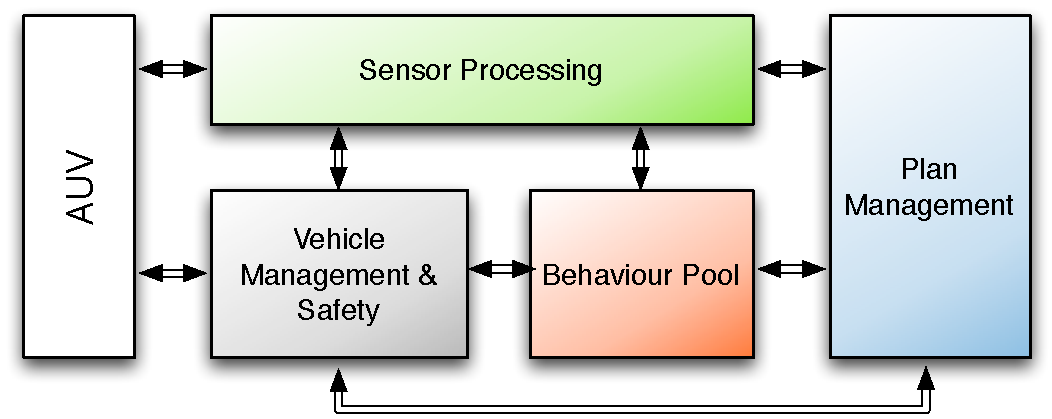
\includegraphics[width=0.9\columnwidth]{sw_arch_overview}
	\caption{High-level view of the FlatFish control architecture}
	\label{fig:sw_arch}
\end{figure}

\subsection{Simulation}

Using Gazebo\footnote{http://gazebosim.org/} and OSG Ocean\footnote{https://code.google.com/p/osgocean/}

integration with ROck done in \cite{watanabe2015} see figure~\ref{fig:simulation}

\begin{figure}[!t]
	\centering
	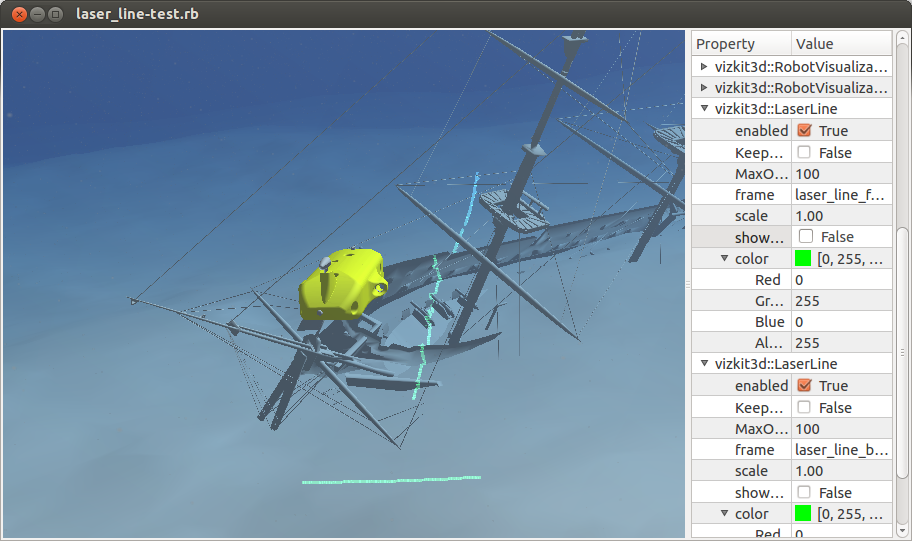
\includegraphics[width=0.9\columnwidth]{flatfish_simulation}
	\caption{Screenshot of the simulation with an active FlatFish using the laser line projectors.}
	\label{fig:simulation}
\end{figure}


\subsection{Navigation System}

\begin{figure}[!t]
\begin{center}
	\subfloat[During transitions the INS/DVL based localisation is supported by tracking of asset strucutres like flowlines ]{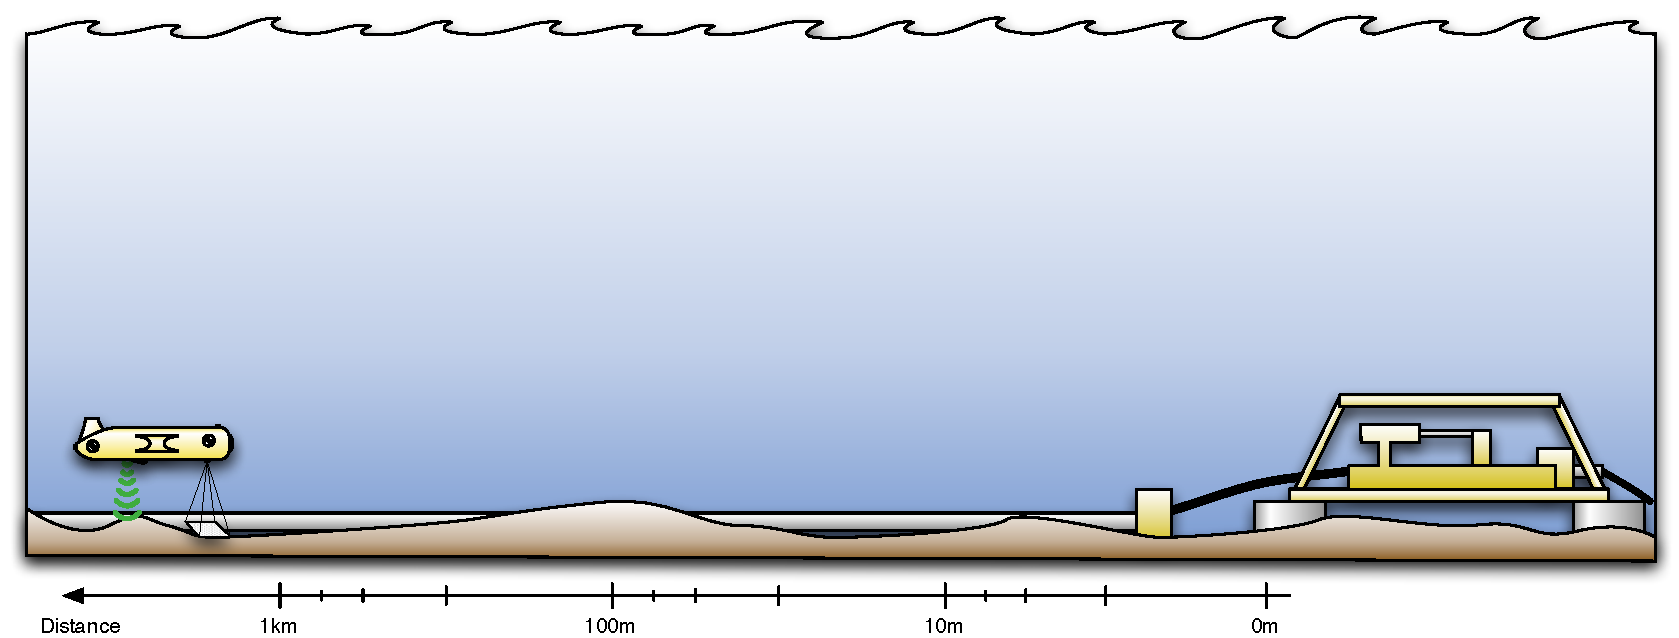
\includegraphics[width=\columnwidth]{FF-NavigationOverview-1}}\\
	\subfloat[Closer (less than 100 m) to major asset structures the forward looking imaging sonar and the obstacle avoidance sonar is used to localise the structure]{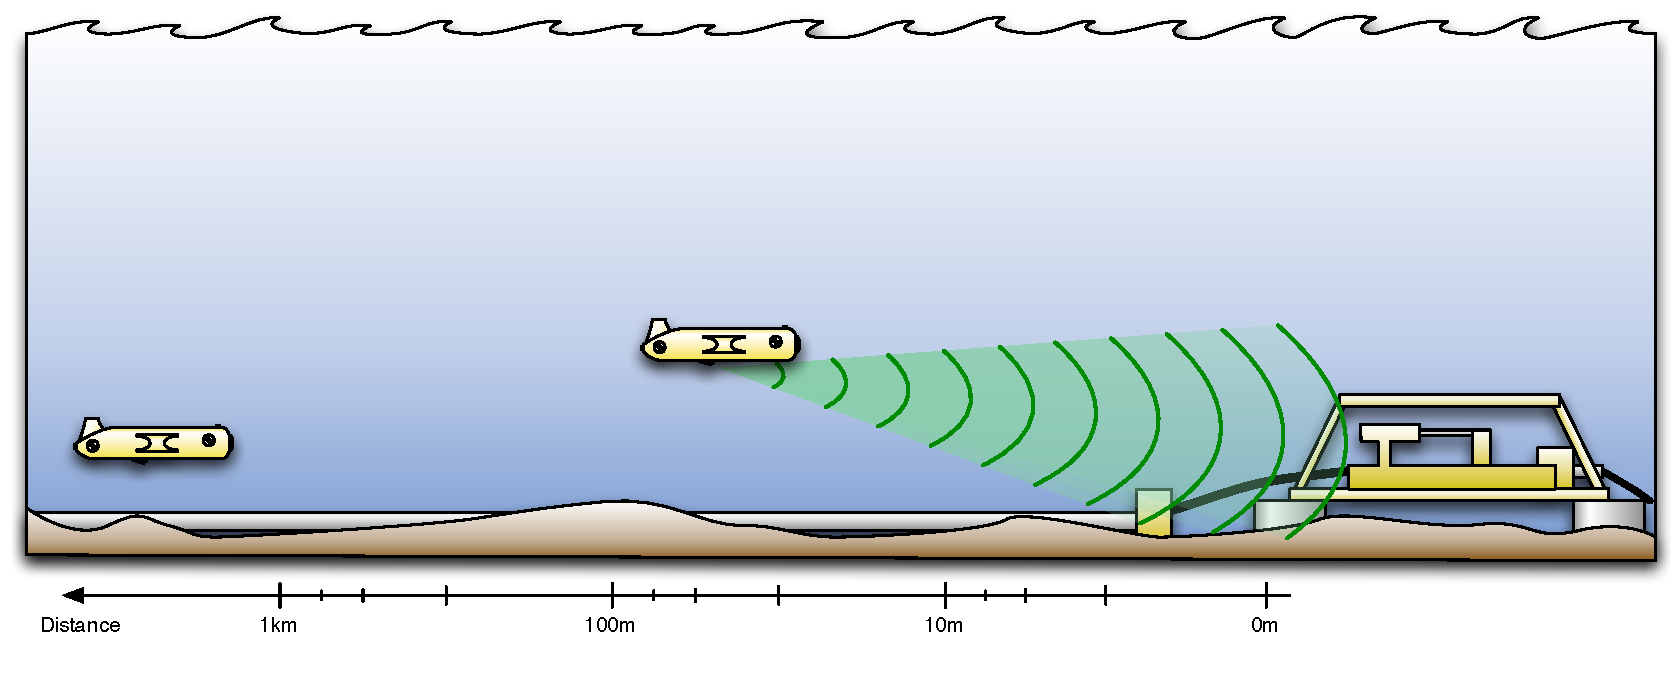
\includegraphics[width=\columnwidth]{FF-NavigationOverview-2}}\\
	\subfloat[During inspection the 3D reconstruction data (visual and sonar) is used to track its relative position to the structure ]{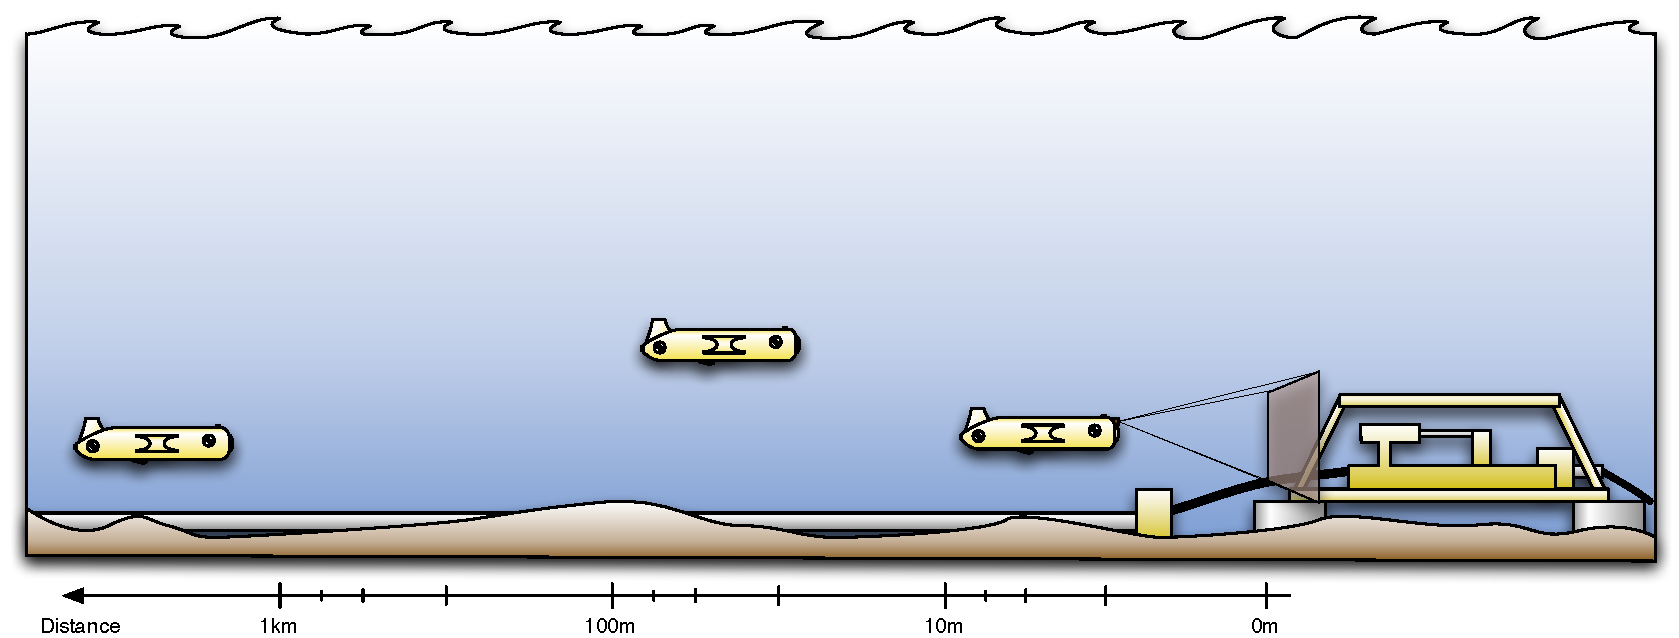
\includegraphics[width=\columnwidth]{FF-NavigationOverview-3}}\\
\caption{Overview of the three major navigation modalities for the layout-supported navigation of FlatFish }
\label{fig:nav_overview}
\end{center}
\end{figure}

\subsection{Inspection System}

Laser line based on \cite{duda2013} teste ind turbid water \cite{albiez2015} and
\cite{mcleod2013}

\begin{figure}[!t]
	\centering
	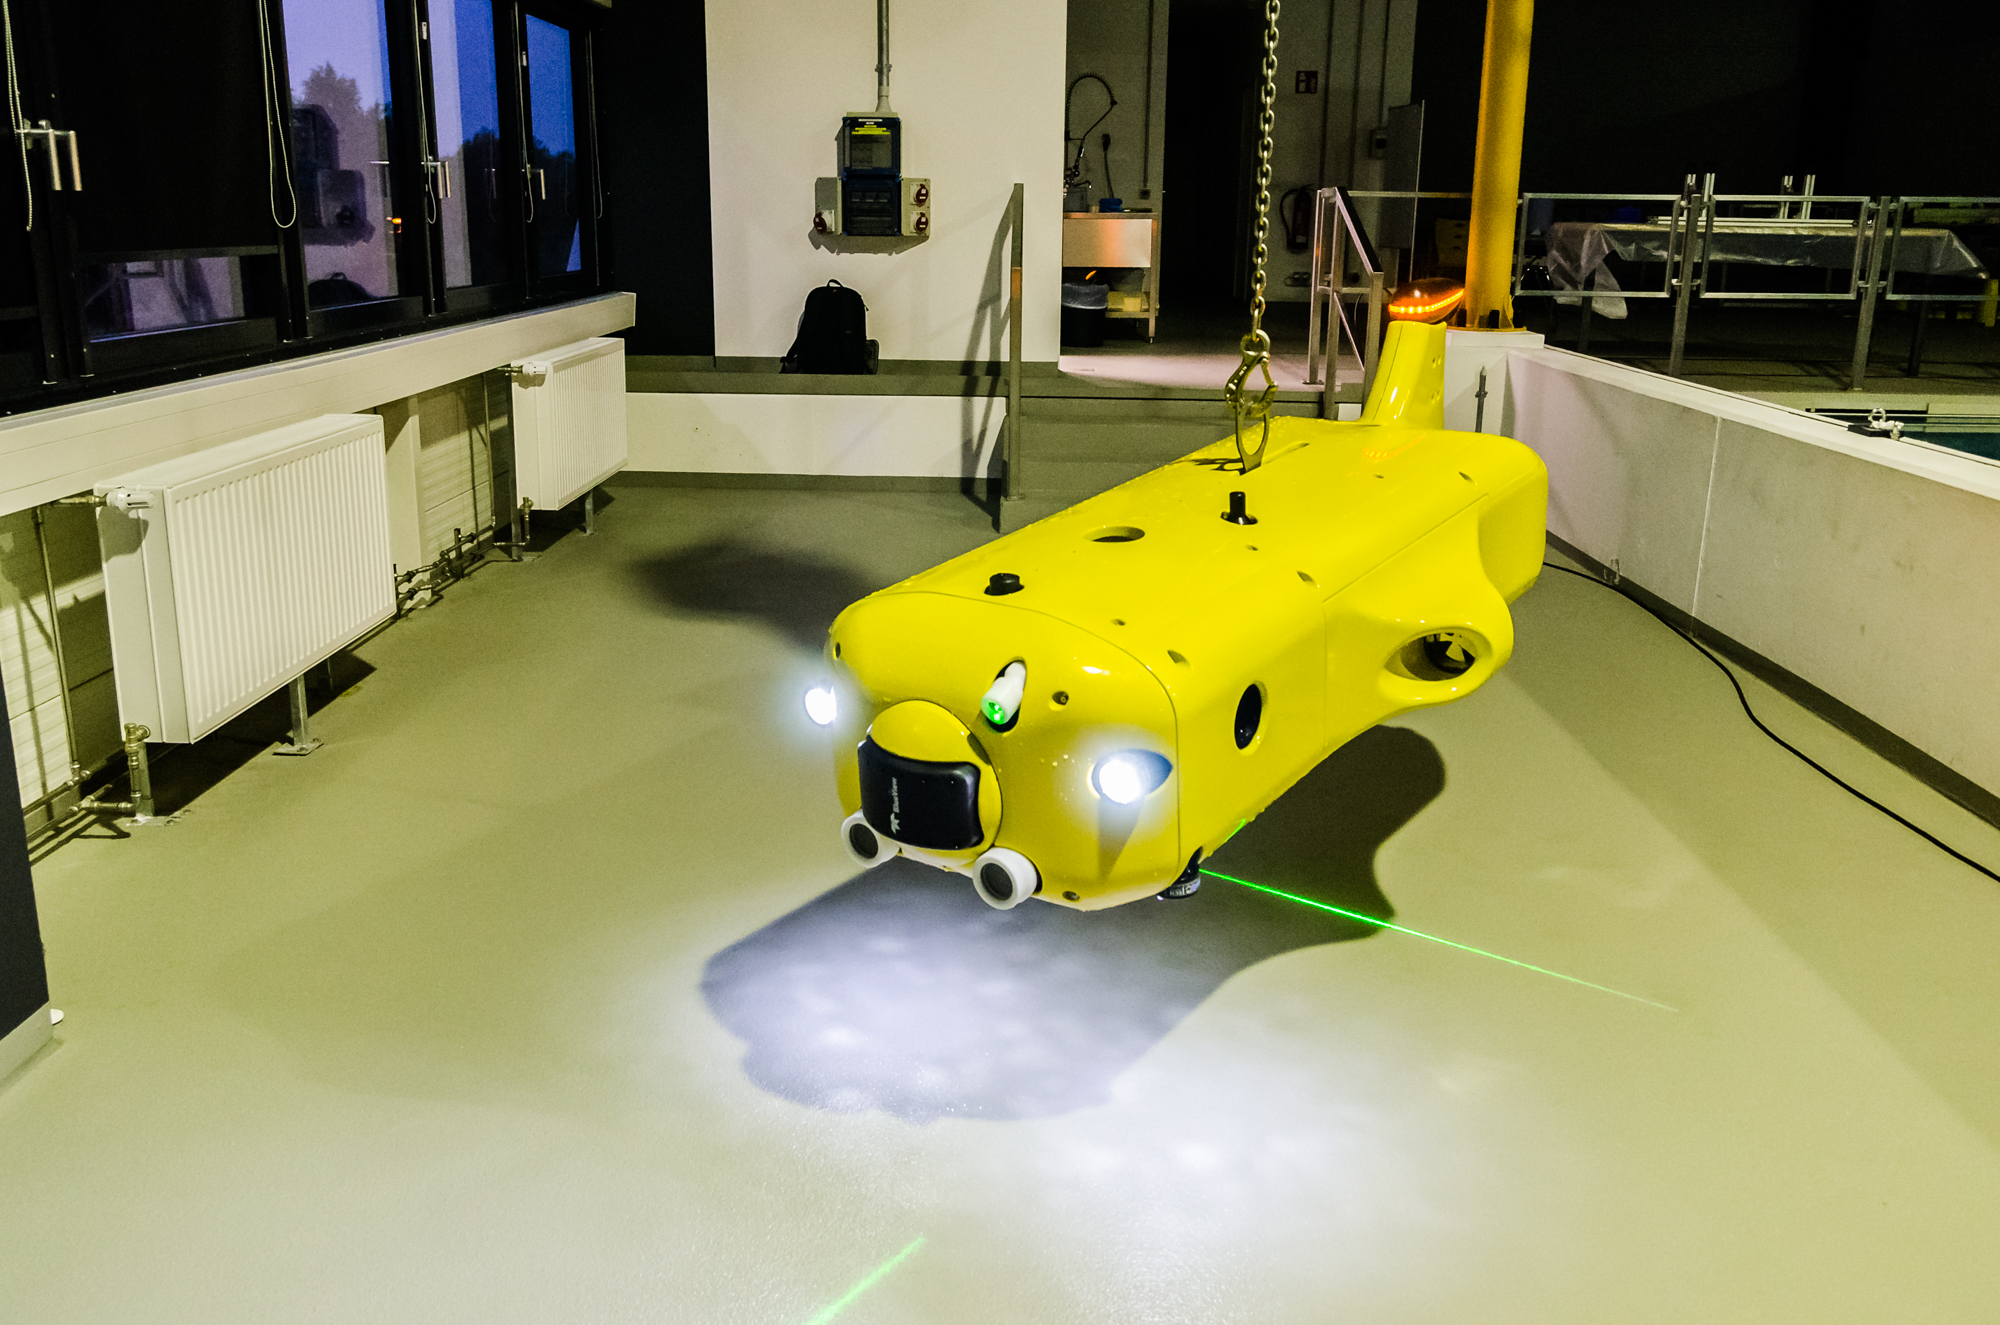
\includegraphics[width=0.9\columnwidth]{FlatFish-3.jpg}
	\caption{FlatFish attached to the crane at DFKI in Bremen. Good visible are the green lines of the laser projectors under and in front of the AUV. On the front part of the AUV the BlueView inspection sonar, the lights and the forward looking stereo camera system is visible.}
	\label{fig:flatfishlaser}
\end{figure}


\section{Integration Tests}

In June 2015 the integration of the first vehicle was finished in Bremen, Germany and a
series of specification compliance tests have been done. The goal of these tests were to
check whether the fully integrated AUV complies to the specifications with respect to the
mechatronic system and the basic motion capabilities. 

\begin{figure}[!t]
	\centering
	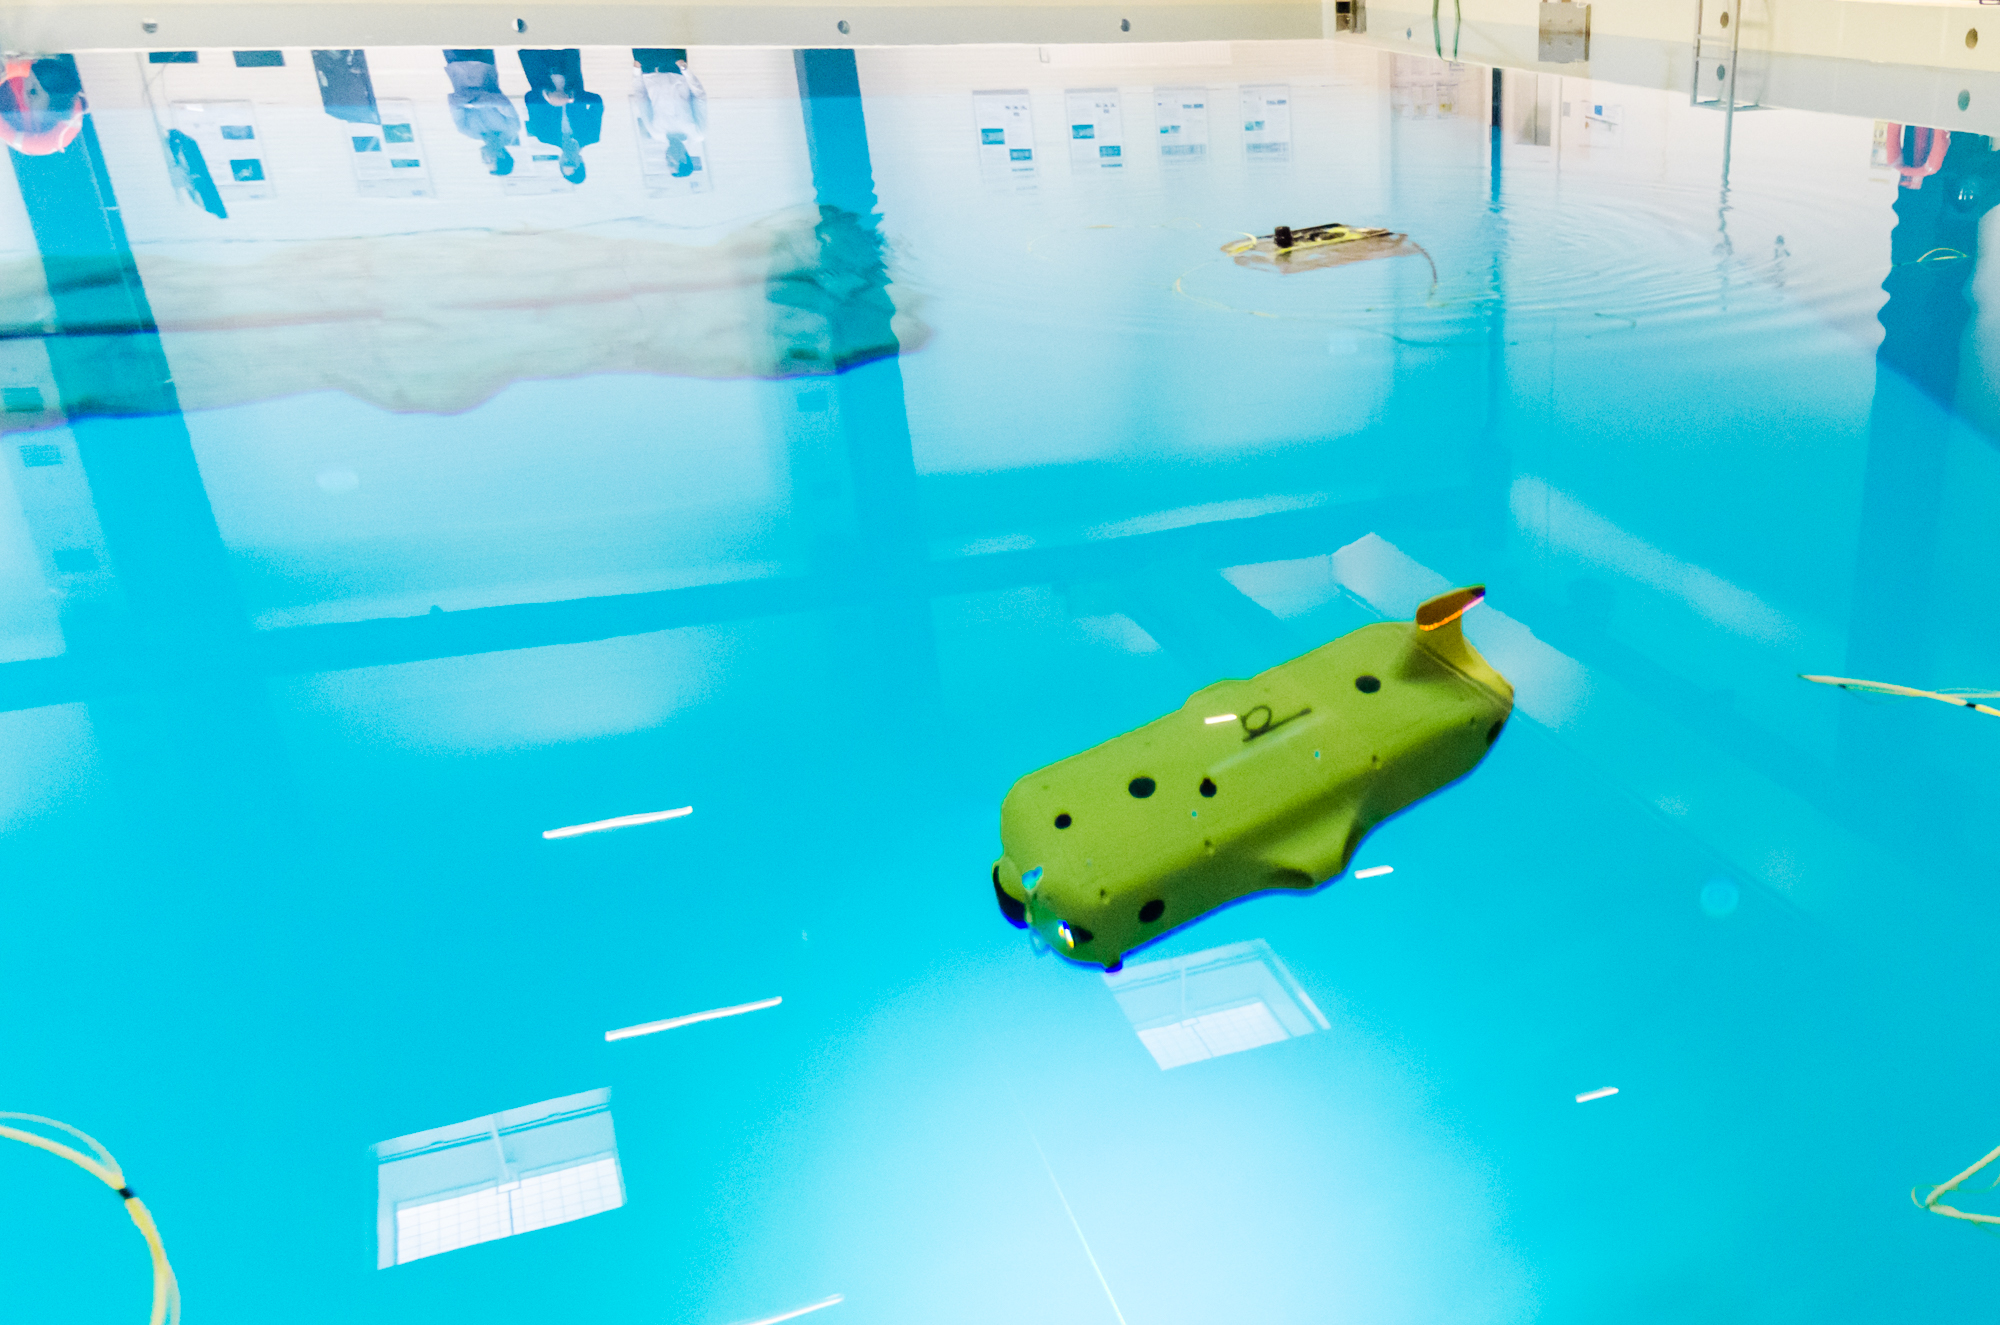
\includegraphics[width=0.9\columnwidth]{FlatFish-2.jpg}
	\caption{FlatFish in the maritime test tank at the DFKI facilities in Bremen during the specification compliance tests. The pipeline mock-up is visible in the top left of the picture.}
	\label{fig:flatfish2}
\end{figure}

The test were done in the large saltwater tank of the maritime exploration hall in Bremen.
A mock-up of a pipeline was installed as a visual target for the vehicle and the
experiments were documented by a Mini-ROV (see figure \ref{fig:flatfish2}). 

The tests consisted in a series of tracks the FlatFish had to follow while using the
INS/DVL based dead-reckoning pose estimator and the way point following behaviour. The
pipeline mock-up was the target for testing the downward looking camera systems and used
as a the test object for the pipeline detector. The FlatFish AUV was able to successfully
fulfill all the parts of the test. The way point navigation autonomously followed a set of
way points within the tank over a time period of 30 minutes. All sensors of FlatFish
worked correctly and the pipeline detector was able to detect the pipeline whenever
FlatFish crossed it. 

\section{Conclusion}

The FlatFish AUV is the first step to an integrated sub-sea resident inspection system for
offshore oil and gas. The specification compliance tests done at the DFKI RIC in Bremen,
Germany showed that the mechatronic design of FlatFish (...)

% conference papers do not normally have an appendix


% use section* for acknowledgement
\section*{Acknowledgment}

The FlatFish project is part of the ongoing research and development program of BG Group
Brasil. It is funded by the Brasilian government via the Agencia Nacional do Petroleo, Gas
Natural e Biocombustiveis (ANP) and, due to its high innovative nature, co-funded by the
EMPRAPII (Empresa Brasileira de Pesquisa e Inovacao Industrial) program. 

The authors would like to thank BG Group for the excellent support of the project, with
special thanks to Gordon Laurenson, Phil Bremner, Diana Charles, Rosane Zagatti and John
Costin.

% references section

\bibliographystyle{IEEEtran}
\bibliography{IEEEabrv,OCEANS2015_Washington_FlatrFish}



% that's all folks
\end{document}


